\chapter{Κώδικας εφαρμογής του αλγορίθμου \textlatin{Bayes}} 
\vfil\vfil\null

\begin{center}
    \includegraphics[width=1.0\linewidth,page=1]{Figures/Final Code Illustration-Bayesian.pdf}
\end{center}

%\begin{left}
    \includegraphics[width=1.0\linewidth,page=2]{Figures/Final Code Illustration-Bayesian.pdf}
%\end{left}

\begin{center}
    \includegraphics[width=1.0\linewidth,page=3]{Figures/Final Code Illustration-Bayesian.pdf}
\end{center}

\begin{center}
    \includegraphics[width=1.0\linewidth,page=4]{Figures/Final Code Illustration-Bayesian.pdf}
\end{center}

\begin{center}
    \includegraphics[width=1.0\linewidth,page=5]{Figures/Final Code Illustration-Bayesian.pdf}
\end{center}

\begin{center}
    \includegraphics[width=1.0\linewidth,page=6]{Figures/Final Code Illustration-Bayesian.pdf}
\end{center}
%\section{Υπολογισμός της \textlatin{NXSV} από φωτομετρικά δεδομένα}
%\section{Υπολογισμός της λαμπρότητας}
%\section{Εφαρμογή του αλγορίθμου \textlatin{Bayes}}
%\usepackage{pdfpages}
%\includepdf[pages=-]{Final Code Illustration-Bayesian.pdf}
